% 若编译失败,且生成 .synctex(busy) 辅助文件,可能有两个原因:
% 1. 需要插入的图片不存在:Ctrl + F 搜索 'figure' 将这些代码注释/删除掉即可
% 2. 路径/文件名含中文或空格:更改路径/文件名即可

% --------------------- 文章宏包及相关设置 --------------------- %
% >> ------------------ 文章宏包及相关设置 ------------------ << %
% 设定文章类型与编码格式
\documentclass[UTF8]{article}		

% 物理实验报告所需的其它宏包
\usepackage{ulem}   % \uline 下划线支持
\usepackage{circuitikz} % 电路图 tikz 支持
\usepackage{pdfpages}   % 用于导入 pdf 文件
\usepackage{multirow}   % 用于表格合并单元格

% 本 .tex 专属的宏定义
    \def\V{\ \mathrm{V}}
    \def\uV{\ \mu\mathrm{V}}
    \def\mV{\ \mathrm{mV}}
    \def\K{\ \mathrm{K}}
    \def\kV{\ \mathrm{KV}}
    \def\KV{\ \mathrm{KV}}
    \def\MV{\ \mathrm{MV}}
    \def\uA{\ \mu\mathrm{A}}
    \def\mA{\ \mathrm{mA}}
    \def\A{\ \mathrm{A}}
    \def\kA{\ \mathrm{KA}}
    \def\KA{\ \mathrm{KA}}
    \def\MA{\ \mathrm{MA}}
    \def\O{\ \Omega}
    \def\mO{\ \Omega}
    \def\kO{\ \mathrm{K}\Omega}
    \def\KO{\ \mathrm{K}\Omega}
    \def\MO{\ \mathrm{M}\Omega}
    \def\Hz{\ \mathrm{Hz}}
    \def\uF{\ \mu\mathrm{F}}
    \def\mF{\ \mathrm{mF}}
    \def\F{\ \mathrm{F}}
    \def\Re{\mathrm{\,Re}\,}
    \def\Im{\mathrm{\,Im}\,}
    \def\sinc{\mathrm{\,sinc}\,}

% 自定义宏定义
    \def\N{\mathbb{N}}
    \def\F{\mathbb{F}}
    \def\Z{\mathbb{Z}}
    \def\Q{\mathbb{Q}}
    \def\R{\mathbb{R}}
    \def\C{\mathbb{C}}
    \def\T{\mathbb{T}}
    \def\S{\mathbb{S}}
    %\def\A{\mathbb{A}}
    \def\I{\mathscr{I}}
    \def\d{\mathrm{d}}
    \def\p{\partial}


% 导入基本宏包
    \usepackage[UTF8]{ctex}     % 设置文档为中文语言
    \usepackage{hyperref}  % 宏包:自动生成超链接 (此宏包与标题中的数学环境冲突)
    \hypersetup{
        colorlinks=true,    % false:边框链接 ; true:彩色链接
        citecolor={blue},    % 文献引用颜色
        linkcolor={blue},   % 目录 (我们在目录处单独设置),公式,图表,脚注等内部链接颜色
        urlcolor={orange},    % 网页 URL 链接颜色,包括 \href 中的 text
        % cyan 浅蓝色 
        % magenta 洋红色
        % yellow 黄色
        % black 黑色
        % white 白色
        % red 红色
        % green 绿色
        % blue 蓝色
        % gray 灰色
        % darkgray 深灰色
        % lightgray 浅灰色
        % brown 棕色
        % lime 石灰色
        % olive 橄榄色
        % orange 橙色
        % pink 粉红色
        % purple 紫色
        % teal 蓝绿色
        % violet 紫罗兰色
    }
    % \usepackage{docmute}    % 宏包:子文件导入时自动去除导言区,用于主/子文件的写作方式,\include{./51单片机笔记}即可。注:启用此宏包会导致.tex文件capacity受限。
    \usepackage{amsmath}    % 宏包:数学公式
    \usepackage{mathrsfs}   % 宏包:提供更多数学符号
    \usepackage{amssymb}    % 宏包:提供更多数学符号
    \usepackage{pifont}     % 宏包:提供了特殊符号和字体
    \usepackage{extarrows}  % 宏包:更多箭头符号 
    \usepackage{multicol}   % 宏包:支持多栏 

% 文章页面margin设置
    \usepackage[a4paper]{geometry}
        \geometry{top=0.75in}
        \geometry{bottom=0.75in}
        \geometry{left=0.75in}
        \geometry{right=0.75in}   % 设置上下左右页边距
        \geometry{marginparwidth=1.75cm}    % 设置边注距离(注释、标记等)

% 配置数学环境
    \usepackage{amsthm} % 宏包:数学环境配置
    % theorem-line 环境自定义
        \newtheoremstyle{MyLineTheoremStyle}% <name>
            {11pt}% <space above>
            {11pt}% <space below>
            {\kaishu}% <body font> 默认使用正文字体, \kaishu 为楷体
            {}% <indent amount>
            {\bfseries}% <theorem head font> 设置标题项为加粗
            {:\ \ }% <punctuation after theorem head>
            {.5em}% <space after theorem head>
            {\textbf{#1}\thmnumber{#2}\ \ (\,\textbf{#3}\,)}% 设置标题内容顺序
        \theoremstyle{MyLineTheoremStyle} % 应用自定义的定理样式
        \newtheorem{LineTheorem}{Theorem.\,}
    % theorem-block 环境自定义
        \newtheoremstyle{MyBlockTheoremStyle}% <name>
            {11pt}% <space above>
            {11pt}% <space below>
            {\kaishu}% <body font> 使用默认正文字体
            {}% <indent amount>
            {\bfseries}% <theorem head font> 设置标题项为加粗
            {:\\ \indent}% <punctuation after theorem head>
            {.5em}% <space after theorem head>
            {\textbf{#1}\thmnumber{#2}\ \ (\,\textbf{#3}\,)}% 设置标题内容顺序
        \theoremstyle{MyBlockTheoremStyle} % 应用自定义的定理样式
        \newtheorem{BlockTheorem}[LineTheorem]{Theorem.\,} % 使用 LineTheorem 的计数器
    % definition 环境自定义
        \newtheoremstyle{MySubsubsectionStyle}% <name>
            {11pt}% <space above>
            {11pt}% <space below>
            {}% <body font> 使用默认正文字体
            {}% <indent amount>
            {\bfseries}% <theorem head font> 设置标题项为加粗
            {:\\ \indent}% <punctuation after theorem head>
            {0pt}% <space after theorem head>
            {\textbf{#3}}% 设置标题内容顺序
        \theoremstyle{MySubsubsectionStyle} % 应用自定义的定理样式
        \newtheorem{definition}{}

%宏包:有色文本框(proof环境)及其设置
    \usepackage{xcolor}    %设置插入的文本框颜色
    \usepackage[strict]{changepage}     % 提供一个 adjustwidth 环境
    \usepackage{framed}     % 实现方框效果
        \definecolor{graybox_color}{rgb}{0.95,0.95,0.96} % 文本框颜色。修改此行中的 rgb 数值即可改变方框纹颜色,具体颜色的rgb数值可以在网站https://colordrop.io/ 中获得。(截止目前的尝试还没有成功过,感觉单位不一样)(找到喜欢的颜色,点击下方的小眼睛,找到rgb值,复制修改即可)
        \newenvironment{graybox}{%
        \def\FrameCommand{%
        \hspace{1pt}%
        {\color{gray}\vrule width 2pt}%
        {\color{graybox_color}\vrule width 4pt}%
        \colorbox{graybox_color}%
        }%
        \MakeFramed{\advance\hsize-\width\FrameRestore}%
        \noindent\hspace{-4.55pt}% disable indenting first paragraph
        \begin{adjustwidth}{}{7pt}%
        \vspace{2pt}\vspace{2pt}%
        }
        {%
        \vspace{2pt}\end{adjustwidth}\endMakeFramed%
        }

% 外源代码插入设置
    % matlab 代码插入设置
    \usepackage{matlab-prettifier}
        \lstset{style=Matlab-editor}    % 继承 matlab 代码高亮 , 此行不能删去
    \usepackage[most]{tcolorbox} % 引入tcolorbox包 
    \usepackage{listings} % 引入listings包
        \tcbuselibrary{listings, skins, breakable}
        \newfontfamily\codefont{Consolas} % 定义需要的 codefont 字体
        \lstdefinestyle{MatlabStyle_inc}{   % 插入代码的样式
            language=Matlab,
            basicstyle=\footnotesize\ttfamily\codefont,    % ttfamily 确保等宽 
            breakatwhitespace=false,
            breaklines=true,
            captionpos=b,
            keepspaces=true,
            numbers=left,
            numbersep=15pt,
            showspaces=false,
            showstringspaces=false,
            showtabs=false,
            tabsize=2,
            xleftmargin=15pt,   % 左边距
            %frame=single, % single 为包围式单线框
            frame=shadowbox,    % shadowbox 为带阴影包围式单线框效果
            %escapeinside=``,   % 允许在代码块中使用 LaTeX 命令 (此行无用)
            %frameround=tttt,    % tttt 表示四个角都是圆角
            framextopmargin=0pt,    % 边框上边距
            framexbottommargin=0pt, % 边框下边距
            framexleftmargin=5pt,   % 边框左边距
            framexrightmargin=5pt,  % 边框右边距
            rulesepcolor=\color{red!20!green!20!blue!20}, % 阴影框颜色设置
            %backgroundcolor=\color{blue!10}, % 背景颜色
        }
        \lstdefinestyle{MatlabStyle_src}{   % 插入代码的样式
            language=Matlab,
            basicstyle=\small\ttfamily\codefont,    % ttfamily 确保等宽 
            breakatwhitespace=false,
            breaklines=true,
            captionpos=b,
            keepspaces=true,
            numbers=left,
            numbersep=15pt,
            showspaces=false,
            showstringspaces=false,
            showtabs=false,
            tabsize=2,
        }
        \newtcblisting{matlablisting}{
            %arc=2pt,        % 圆角半径
            % 调整代码在 listing 中的位置以和引入文件时的格式相同
            top=0pt,
            bottom=0pt,
            left=-5pt,
            right=-5pt,
            listing only,   % 此句不能删去
            listing style=MatlabStyle_src,
            breakable,
            colback=white,   % 选一个合适的颜色
            colframe=black!0,   % 感叹号后跟不透明度 (为 0 时完全透明)
        }
        \lstset{
            style=MatlabStyle_inc,
        }

% table 支持
    \usepackage{booktabs}   % 宏包:三线表
    \usepackage{tabularray} % 宏包:表格排版
    \usepackage{longtable}  % 宏包:长表格

% figure 设置
    \usepackage{graphicx}  % 支持 jpg, png, eps, pdf 图片 
    \usepackage{svg}       % 支持 svg 图片
        \svgsetup{
            % 指向 inkscape.exe 的路径
            inkscapeexe = C:/aa_MySame/inkscape/bin/inkscape.exe, 
            % 一定程度上修复导入后图片文字溢出几何图形的问题
            inkscapelatex = false                 
        }
    \usepackage{subcaption} % 用于子图和小图注  

% 图表进阶设置
    \usepackage{caption}    % 图注、表注
        \captionsetup[figure]{name=图}  
        \captionsetup[table]{name=表}
        \captionsetup{
            labelfont=bf, % 设置标签为粗体
            textfont=bf,  % 设置文本为粗体
            font=small  
        }
    \usepackage{float}     % 图表位置浮动设置 
    \usepackage{etoolbox} % 用于保证图注表注的数学字符为粗体
        \AtBeginEnvironment{figure}{\boldmath} % 图注中的数学字符为粗体
        \AtBeginEnvironment{table}{\boldmath}  % 表注中的数学字符为粗体
        \AtBeginEnvironment{tabular}{\unboldmath}   % 保证表格中的数学字符不受额外影响

% 圆圈序号自定义
    \newcommand*\circled[1]{\tikz[baseline=(char.base)]{\node[shape=circle,draw,inner sep=0.8pt, line width = 0.03em] (char) {\bfseries #1};}}   % TikZ solution

% 列表设置
    \usepackage{enumitem}   % 宏包:列表环境设置
        \setlist[enumerate]{
            label=(\arabic*) ,   % 设置序号样式为加粗的 (1) (2) (3)
            ref=\arabic*, % 如果需要引用列表项,这将决定引用格式(这里仍然使用数字)
            itemsep=0pt, parsep=0pt, topsep=0pt, partopsep=0pt, leftmargin=3.5em} 
        \setlist[itemize]{itemsep=0pt, parsep=0pt, topsep=0pt, partopsep=0pt, leftmargin=3.5em}
        \newlist{circledenum}{enumerate}{1} % 创建一个新的枚举环境  
        \setlist[circledenum,1]{  
            label=\protect\circled{\arabic*}, % 使用 \arabic* 来获取当前枚举计数器的值,并用 \circled 包装它  
            ref=\arabic*, % 如果需要引用列表项,这将决定引用格式(这里仍然使用数字)
            itemsep=0pt, parsep=0pt, topsep=0pt, partopsep=0pt, leftmargin=3.5em
        }  

% 其它设置
    % 脚注设置
        \renewcommand\thefootnote{\ding{\numexpr171+\value{footnote}}}
    % 参考文献引用设置
        \bibliographystyle{unsrt}   % 设置参考文献引用格式为unsrt
        \newcommand{\upcite}[1]{\textsuperscript{\cite{#1}}}     % 自定义上角标式引用
    % 文章序言设置
        \newcommand{\cnabstractname}{序言}
        \newenvironment{cnabstract}{%
            \par\Large
            \noindent\mbox{}\hfill{\bfseries \cnabstractname}\hfill\mbox{}\par
            \vskip 2.5ex
            }{\par\vskip 2.5ex}

% 文章默认字体设置
    \usepackage{fontspec}   % 宏包:字体设置
        \setmainfont{SimSun}    % 设置中文字体为宋体字体
        \setCJKmainfont[AutoFakeBold=3]{SimSun} % 设置加粗字体为 SimSun 族,AutoFakeBold 可以调整字体粗细
        \setmainfont{Times New Roman} % 设置英文字体为Times New Roman

% 各级标题自定义设置
    \usepackage{titlesec}   
        % section标题自定义设置 
        \titleformat{\section}[hang]{\normalfont\Large\bfseries\boldmath}{\thesection}{8pt}{}
        % subsection 标题自定义设置
        \titleformat{\subsection}[hang]{\normalfont\large\bfseries\boldmath}{\thesubsection}{8pt}{}
        \titlespacing*{\subsection}{0pt}{10pt}{6pt} % 控制上下间距


% --------------------- 文章宏包及相关设置 --------------------- %
% >> ------------------ 文章宏包及相关设置 ------------------ << %


% ------------------------ 文章信息区 ------------------------ %
% ------------------------ 文章信息区 ------------------------ %
% 页眉页脚设置
\usepackage{fancyhdr}   %宏包:页眉页脚设置
    \pagestyle{fancy}
    \fancyhf{}
    \cfoot{\thepage}
    \renewcommand\headrulewidth{1pt}
    \renewcommand\footrulewidth{0pt}
    \rhead{\bfseries \large {\color{red} 分组序号: 2-05}}    
    \chead{《基础物理实验》实验报告,\ 丁毅,\ 2023K8009908031}
    \lhead{\small Ex.01 杨氏模量 (2024.11.12)}

% 开始编辑文章

\begin{document}
\begin{center}\large
    \vspace*{-0.8cm}
    \noindent{\huge\bfseries《\ \ 基\ \ 础\ \ 物\ \ 理\ \ 实\ \ 验\ \ \ 》\ \ 实\ \ 验\ \ 报\ \ 告 }
    \\\vspace{0.1cm}
    \noindent{
    {\bfseries 
    实验名称:\uline{\hspace{1.3cm} 杨氏模量与微小量测量 \hspace{1.3cm}}
    }\hspace{0.4cm}
    指导教师:\uline{\hspace{0.5cm}董政 \ \ dongz@ihep.ac.cn\hspace{0.5cm}}
    }
    \\\vspace{0.1cm}
    \noindent
    {
    姓名:\uline{\,\,\,丁毅\,\,\,}\hspace{0.2cm}
    学号:\uline{\,\,\,{ 2023K8009908031}\,\,\,}\hspace{0.2cm}
    班级/专业:\uline{\,\,\,{2308/电子信息}\,\,\,}\hspace{0.2cm}
    分组序号:\uline{\,\,\,{2-05}\,\,\,}
    }
    \\\vspace{0.1cm}
    \noindent{
    实验日期:\uline{\,\,{ 2024.11.12}\,\,}\hspace{0.2cm}
    实验地点:\uline{\,\,\,教学楼{ 710}\,\,\,}\hspace{0.2cm}
    是否调课/补课:\uline{\hspace{0.26cm}否 \hspace{0.26cm}}\hspace{0.2cm}
    成绩:\uline{\hspace{2cm}}
    }
\end{center}
\vspace{-0.4cm}
\noindent\rule{\textwidth}{0.075em}   % 分割线
\vspace{-1.0cm}

% 目录
\setcounter{tocdepth}{2}  % 目录深度为 2(不显示 subsubsection)
\noindent\tableofcontents\thispagestyle{fancy}   % 显示页码、页眉等
\newpage
\rhead{\bfseries\small 分组序号: 2-05}
% ------------------------ 文章信息区 ------------------------ %
% ------------------------ 文章信息区 ------------------------ %


%% 下面是正文内容


\section{实验目的}
\begin{enumerate}
\item 理解测量杨氏模量的静态法和动态法的相关原理,尤其是前者各种方法对测量微小位移的优缺点;
\item 熟悉霍尔位置传感器的特性,理解传感器相关曲线的意义;
\item 了解光杠杆法的原理和适用范围;
\item 学会对一些实验器材的规范调节,比如读数望远镜、读数显微镜等;
\item 学习用逐差法、作图法和最小二乘法处理数据;
\item 学会计算各物理量的不确定度,并用不确定度正确表达实验结果。
\end{enumerate}

\section{数据的不确定度}

本次实验的一大重点就是理解并掌握数据的有效数字及不确定度的计算与合成,
故专门开一小节讨论。

\subsection*{6.1 \ 不确定度 $\Delta N$}

用以表示测量值不确定的程度,
反应数据的可信度,是测量结果质量的指标。测量结果一般表示为$Y=N+\Delta N$的形式,并且将$\Delta N/N$称为数据的相对不确定度。

\subsection*{6.2 \ 两类不确定度(A 类与 B 类)}


A类不确定度$u_A(x)$:即用以表示同样环境条件下多次
估读测量造成的不确定度(也称为标准偏差),表示为:
\begin{equation}
   u_A(x)=\sqrt{\frac{\sum_{i=1}^n(x_i-\overline x)^2}{n(n-1)}}
\end{equation}

B类不确定度$u_B(x)$:又分为单次测量时估读造成的不确定度$u_{B1}(x)$与仪器不确定度$u_{B2}(x)$,表示为:
\begin{equation}
   u_{B1}(x)=d,\ \frac{d}{10},\ \frac{d}{5}\qquad u_{B2}(x)=\frac{e}{\sqrt 3} 
\end{equation}
本次实验中取$u_{B1}(x)=\frac{d}{10}$,其中$d$为仪器最小分度值,$e$为仪器所示的最大误差,也称为允差。

\subsection*{6.3 \ 不确定度的合成}


单次测量时:
\begin{equation}
    u(x)=\sqrt{u_{B1}^2(x)+u^2_{B2}(x)} 
\end{equation}
特别地,在长度测量中,因为读数是两个位置之差,故
\begin{equation}
    u(x)=\sqrt{u_{B1}^2(x)+u_{B1}^2(x)+u^2_{B2}(x)} =\sqrt{2u_{B1}^2(x)+u^2_{B2}(x)} 
\end{equation}

多次测量时:
\begin{equation}
   u(x)=\sqrt{u_A^2(x)+u^2_{B2}(x)} 
\end{equation}


\section{拉伸法}
\subsection{实验仪器与用具}

CCD 杨氏弹性模量测量仪(LB-YM1 型、YMC-2 型)、螺旋测微器、钢卷尺等。

其主要技术指标如下:采用
分划板(刻度范围 4mm,分度值 0.05mm,设有限位槽,可防止来回摆动,
采用LED 照明)+
CCD测量显微镜系统(放大倍率60倍,内含电子刻度线,可二维调节,
可卸下用于其他微位移测量场合)+
彩色液晶监视器方案。
\begin{figure}[H]\centering
    \includegraphics[width=0.4\columnwidth]{assets/0/da2dd09fb93428ae0fb1bc23c8c81af2.png}
    \caption{LB-YM1 型实验装置}
\end{figure}



\subsection{实验原理}
物体在外力作用下都会发生形变。当形变在一定限度内,撤走外力能恢复原状的形变称为弹性形变。
反之撤走外力之后仍有剩余形变,称为塑性形变。发生弹性形变时,弹性模量便是反应材料形变与内应力关系的基本物理量。

设柱状物体的长度为$L$,截面积为$S$,沿长度方向受外力$F$作用后伸长(或缩短)量为$\Delta L$,单位横截面积上垂
直作用力$F/S$称为正应力,物体的相对伸长$\Delta L/L$称为线应变。胡克定律告诉我们:
\begin{equation}
   F/S=Y\frac{\Delta L}{L} 
\end{equation}
其中$Y$便称为杨氏模量,本实验中我们将以显微镜和CCD成像系统进行对$\Delta L$的测量,并通过砝码测量外力,通过钢卷尺测量金属丝长度,
通过螺旋测微器测量金属丝直径,从而将知道有公式:
\begin{equation}
    Y=\frac{4FL}{\pi d^2\Delta L}
\end{equation}

\subsection{实验注意事项}
\begin{enumerate}
\item 需保证分划板卡在下衡梁的槽内,避免其在拉直过程中旋转。

\item 轻轻加减砝码,防止使砝码盘产生微小振动而造成读数起伏较大,或者钼丝突然受力而断裂。

\item 多次测量数据并求平均,包括叉丝读数,金属丝长度和直径等,读数需等刻度值稳定后。

\item CCD器件不可正对太阳、激光或其他强光源。注意保护镜头,防
潮、防尘、防污染。

\item 金属丝必须保持铅直形态。测直径时要特别谨慎,避免由于扭转、拉扯、牵挂导致细丝
折弯变形。

\item 做完实验后归类收纳好各种实验器材。
\end{enumerate}

\subsection{实验步骤}
\begin{enumerate}
\item 仪器调整——例如工作台调平、金属丝安装、夹头调整以及其他实验设备的连接。
打开CCD并进行显微镜的调节,利用磁力滑座与三维调整台在屏幕上先调出数字分划板及十字叉丝,接着进行显微镜的对焦与对准十字叉丝(使之尽量与读数轴平行)。

\item 测量与数据记录——测量钼丝的几何尺寸(有效长度、直径等)。
随后将砝码依次放置并读取数值(等待CCD成像稳定后,可能还需要重新对焦),
再依次取下并读取数值.加减砝码时,
动作要轻,防止因增减砝码时使砝码盘产生微小振动而造成读数起伏较大。
而且不要晃桌子,以免晃动后分划板倾斜造成读数的较大误差。

\item 实验结束后归类收纳好各种实验器材.
\end{enumerate}

\subsection{数据处理}


实验中利用钢卷尺测得钼丝的长度 $L = 791.2$ mm,而钢卷尺的分度值 $d = 1$ mm,允差 $e = \pm 2.0$ mm。长度测量为单次测量,利用 B 类不确定度,得到:
\begin{gather}
u_{B1} = \frac{d}{10} = 0.1 \ \mathrm{mm} ,\quad 
u_{B2} = \frac{e}{\sqrt{3}} = \frac{2.0}{\sqrt{3}} \ \mathrm{mm} \\
\Longrightarrow 
u(L) = \sqrt{2u_{B1}^2 + u_{B2}^2} = \sqrt{2\times 0.1^2 + \left(\frac{2.0}{\sqrt{3}}\right)^2} \ \mathrm{mm} \approx 1.1633 \ \mathrm{mm}
\end{gather}
由于不确定度需保留一位有效数字(只进不退),且测量结果只能有一位可疑数字,钼丝长度应表示为:
\begin{gather}
L = (791 \pm 2) \ \mathrm{mm}
\end{gather}
实验中钼丝直径 $d$ 的测量结果如表 \ref{钼丝直径测量结果} 所示:
\begin{table}[H]\centering
    %\renewcommand{\arraystretch}{1.5} % 调整行间距为 1.5 倍
    %\setlength{\tabcolsep}{1.5mm} % 调整列间距
    \caption{钼丝直径测量结果}
    \label{钼丝直径测量结果}
\begin{tabular}{cccccccccc}\toprule
    序号 & 1 & 2 & 3 & 4 & 5 & 6 & 平均值 $\bar{d}$  \\
    \midrule
    $d$ (mm)  & 0.192 & 0.192 &	0.190 &	0.191 &	0.191 &	0.192 & 0.19133  \\
    \bottomrule
\end{tabular}
\end{table}
直径平均值 $\bar{d}$ 也应取三位有效数字,得到:
\begin{equation}
\bar{d} = 0.191 \ \mathrm{mm}
\end{equation}
本次测量属于多次测量,测量次数 $n = 6$,需要同时考虑 A、B 两类不确定度。螺旋测微仪允差 $e = \pm 0.004 \ \mathrm{mm}$,故不确定度为:
\begin{gather}
u_A(d) = \sqrt{\frac{\sum_{i=1}^{6}\left(d_i - \bar{d}\right)^2}{6\times (6 - 1)}} ,\quad u_{B2}(d) = \frac{e}{\sqrt{3}} \\ 
\Longrightarrow 
u(d) = \sqrt{u_A^2(d) + u_{B2}^2(d)} = 0.0023 \ \mathrm{mm}
\end{gather}
同样的,保留一位有效数字,则 $u(d) = 0.003 \ \mathrm{mm}$,最终的直径测量结果为:
\begin{equation}
d = (0.191 \pm 0.003) \ \mathrm{mm}
\end{equation}

显微镜初始示数为 $l_0 = 1.00 \ \mathrm{mm}$,具体实验数据详见表 \ref{悬挂法实验数据},我们已在其中进行了一些基本的计算。
\begin{table}[H]\centering
    %\renewcommand{\arraystretch}{1.5} % 调整行间距为 1.5 倍
    %\setlength{\tabcolsep}{1.5mm} % 调整列间距
    \caption{悬挂法实验数据}
    \label{悬挂法实验数据}
    \begin{tabular}{cccccccc} 
        \toprule
        序号 $i$ & 砝码 $M$ (g) &  加载 $l_i$ (mm) & 卸载 $l'_i$ (mm) & 均值 $\bar{l}_i$ (mm)  & $\bar{l}_i M_i$ ($\mathrm{mm}\cdot\mathrm{g}$)  & 差值 $\Delta \bar{l}_s = \bar{l}_{i+4} -\bar{l}_{i} $\\
         \midrule
        1 & 250 & 0.80 & 0.65 &  0.7250 & 181.3 & -0.8500 \\
        2 & 500 & 0.55 & 0.40 &  0.4750 &  237.5 & -0.8250 \\
        3 & 750 & 0.30 & 0.30 &  0.3000 & 225.0 & -0.9000 \\
        4 & 1000 & 0.10 & 0.10 &  0.1000 & 100.0 & -0.9000 \\
        5 & 1250 & -0.10 & -0.15 &  -0.1250 &  -156.2 & -\\
        6 & 1500 & -0.35 & -0.35 &  -0.3500 &  -525.0 &  -\\
        7 & 1750 & -0.60 & -0.60 &  -0.6000 &  -1050.0 &  -\\
        8 & 2000 & -0.80 & - & - &  -1600.0 & - \\
        \bottomrule
        \end{tabular}
\end{table}

使用逐差法计算杨氏模量时,除了知道 $\Delta M = 1000 \ \mathrm{g}$,还需要知道示数差值 $\Delta \bar{l}_i$ 的平均值和不确定度。先计算 $\Delta \bar{l}$ 的均值  $\overline{\Delta \bar{l}}$ : 
\begin{equation}
    \overline{\Delta \bar{l}} = \frac{\sum_{i=1}^{4} \Delta \bar{l_i}}{4} = -0.8688 \ \mathrm{mm}
\end{equation}
$\Delta \bar{l}$ 的测量属于多次测量,次数 $n = 4$,CCD 显微镜的允差 $e = \pm 0.005 \ \mathrm{mm}$。简记 $h = \Delta \bar{l}$,则 $\bar{h} = \overline{\Delta \bar{l}}$,其不确定度为:
\begin{gather}
u_A(h) = \sqrt{\frac{\sum_{i=1}^{4}\left(h_i - \overline{h}\right)^2}{4\times (4 - 1)}} ,\quad u_{B2}(h) = \frac{e}{\sqrt{3}} \\ 
\Longrightarrow
u(h) = \sqrt{u_A^2(h) + u_{B2}^2(h)} = 0.0189 \ \mathrm{mm}
\end{gather}
取一位有效数字,$u(h) = 0.02 \ \mathrm{mm}$,得到 $\Delta l $ 的不确定度表示:
\begin{equation}
\Delta l = ( -0.87 \pm 0.02 ) \ \mathrm{mm},\quad \text{也即\ }\Delta l = (0.87 \pm 0.02 ) \ \mathrm{mm}
\end{equation}

还有部分需要用到的数据,如下:
\begin{equation}
    \overline{M} = 1125 \ \mathrm{g},\quad \sum M = 9000 \ \mathrm{g} ,\quad \bar{\bar{l}} = -0.0344 \ \mathrm{mm},\quad \bar{l} = -0.275 \ \mathrm{mm}
\end{equation}


\subsection{实验结果}

\subsubsection*{3.6.1 \ \ 逐差法}

为方便计算,再次汇总一下逐差法需要的数据:
\begin{gather*}
\Delta M = 1\ \mathrm{kg},\quad g = 9.807 \ \mathrm{m\cdot s^{-2}},\quad L = (791 \pm 2) \ \mathrm{mm},\quad d = (0.191 \pm 0.003) \ \mathrm{mm},\quad \Delta l = (0.87 \pm 0.02 ) \ \mathrm{mm}
\end{gather*}
代入数据,可以得到逐差法的计算结果 $\overline{Y}$,进一步与讲义中钼丝杨氏模量的标准值 $Y_0 = 2.3 \times 10^{11} \ \mathrm{N\cdot m^{-2}}$ 进行比较,可以得到相对误差。结果如下:
\begin{gather}
    \overline{Y} =\frac{4\Delta MgL}{\pi d^{2}\Delta\bar{l}}=1.434\times10^{11}\ \mathrm{N/m^{2}} = 3.1120 \times 10^{11} \ \mathrm{N\cdot m^{-2}} \\
    \Delta Y = \overline{Y}\sqrt{ 4 \left[ \frac{u(d)}{d} \right]^2 + \left[ \frac{u(L)}{L} \right]^2 + \left[ \frac{u(\Delta l)}{\Delta l} \right]^2 } = 0.12139 \times 10^{11}  \ \mathrm{N\cdot m^{-2}}\\
    \Longrightarrow  \boldsymbol{
        Y = \overline{Y} \pm \Delta Y = (3.1 \pm 0.2) \times 10^{11} \ \mathrm{N\cdot m^{-2}}
        ,\quad
        \eta = \frac{Y - Y_0}{Y_0} \times 100\% = 35.3035\% 
    }
\end{gather}


\subsubsection*{3.6.2 \ \ 最小二乘法}

将 $Y = \frac{4\Delta MgL}{\pi d^{2}\Delta\bar{l}}$ 变形为下面式子:
\begin{gather}
\bar{l}_i = \left(\frac{4gL}{\pi d^2 Y}\right) M_i + l_0,\quad 
k = \frac{\sum_{i=1}^{8} \left( \bar{l}_i - \bar{\bar{l}}\right) \left(M_i - \overline{M}\right) }{ \sum_{i=1}^{8}\left(M_i - \overline{M}\right)^2 }
\end{gather}
代入数据,可得杨氏模量的计算值:
\begin{equation}
k = -8.6786 \times 10^{-4} \ \mathrm{m\cdot kg^{-1}} ,\quad  \overline{Y} = \frac{4gL}{\pi d^2 | k |} = 3.1197 \times 10^{11} \ \mathrm{N\cdot m^{-2}}
\end{equation}
仍继承逐差法时的不确定度,与标准值 $Y_0$ 进行比较,得到相对误差:
\begin{equation}\boldmath
    Y = \overline{Y} \pm \Delta Y = (3.1 \pm 0.2) \times 10^{11} \ \mathrm{N\cdot m^{-2}}
    ,\quad
    \eta = \frac{Y - Y_0}{Y_0} \times 100\% = 35.6376\%
\end{equation}

\subsubsection*{3.6.3 \ \ 作图法}

选取拟合函数为 $y = ax + b$,在这里即 $\bar{l} = kM + l_0$,在 Matlab 软件中,用 Bisquare 算法对原数据进行拟合,得到拟合结果与优度:
\begin{gather}
k = - 8.6881 \times 10^{-4} \ \mathrm{m\cdot kg^{-1}},\quad 
\overline{Y} = \frac{4gL}{\pi d^2 | k |} = 3.1162 \times 10^{11} \ \mathrm{N\cdot m^{-2}}
\\ 
R^2 = 0.9983,\quad R^2_{\text{adj}} = 0.9980 ,\quad  \text{SSE} = 0.003434 \ \mathrm{mm^2} ,\quad \text{RMSE} = 0.02392 \ \mathrm{mm}
\end{gather}
在坐标系中作出 $\bar{l}$ 随 $M$ 的变化情况,如下图所示:
\begin{figure}[H]\centering
    \includegraphics[width=0.9\columnwidth]{assets/1 悬挂/2024-11-12_21-13-51.pdf}
    \caption{作图法求杨氏模量}
\end{figure}
取合适的有效数字后,作图法的最终结果可写为:
\begin{equation}\boldmath
Y = (3.1 \pm 0.2) \times 10^{11} \ \mathrm{N\cdot m^{-2}},\quad 
\eta = \frac{Y - Y_0}{Y_0} \times 100\% = 35.4889\%
\end{equation}

由此可见,三种方法得到的结果差别不大。


\section{霍尔法}
\subsection{实验仪器与用具}

杭州大华 DHY-1A 霍尔位置传感器法杨氏模量测定仪:包括底座固定箱、读数显微镜、 SS495A 型集成霍尔位置传感器(灵敏度大于 250$\rm mV/mm$,线性范围为 0 - 2mm)、测试仪、磁体、支架、加力机构等。样品为黄铜条、铸铁条。测试仪由霍尔电压测量系统和电子称加力系统构成,霍尔电压测试分为两个量程,带调零功能;电子称加力系统测量范围$0\sim199.9\,\,{\rm g}$,连续可调,三位半数显。


读数显微镜的技术指标:型号 JC-10 型,目镜放大率 10 倍,目镜测微鼓轮最小分度值为 0.01 mm,物镜放大率为 2 倍,测量范围为 0 - 6 mm,实际读书最小分辨率为 0.005 mm;

霍尔电压表的技术指标:量程 0 - 199.9 mV,分辨率为 0.1 mV


\begin{figure}[H]\centering
\begin{subfigure}[b]{0.4\columnwidth}\centering
    \includegraphics[height=150pt]{assets/0/image (19).png}
    \caption{实验装置图}
\end{subfigure}\hfill
\begin{subfigure}[b]{0.6\columnwidth}\centering
    \includegraphics[height=150pt]{assets/0/image (20).png}
    \caption{实验装置图}
\end{subfigure}
\caption{霍尔法测量杨氏模量}
\end{figure}



\subsection{实验原理}


霍尔元件在磁感应强度为$B$的磁场和电流$I$的作用下,产生霍尔电势差\begin{displaymath}U_H=K\cdot I\cdot B\end{displaymath}而在保持电流不变的情况下,在一个具均匀梯度的磁场下运动时,
输出的霍尔电势差的变化量为\begin{displaymath}\Delta U_H=K\cdot I\cdot \frac{\mathrm{d}B}{\mathrm{d}Z}\Delta Z\end{displaymath}其中上式的$\Delta Z$是位移量,
故而上式表明,
当磁场的梯度变化为恒定时,$\Delta U_H$与$\Delta Z$成正比,而这正是我们进行测量杨氏模量的理论基础:
霍尔电势差和位移量之间存在一一对应的关系,
所以在当位移量不太大的时候,
该一一对应的关系具有良好的线性。


如下图所示,设金属篇在刀口间的长度为$ d $,金属片的厚度为$ a $,宽度为$ b $。

\begin{figure}[H]\centering
    \resizebox{!}{150pt}{
        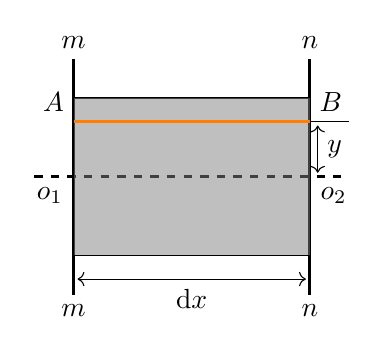
\begin{tikzpicture}
            \draw[dashed,very thick] (-2,0)--(-1.5,0) node[below left]{$ o_1 $}--(1.5,0) node[below right]{$ o_2 $}--(2,0);
            \draw[very thick] (-1.5,-1.5)--(-1.5,1.5);
            \draw[very thick] (1.5,-1.5)--(1.5,1.5);
            \draw (-1.5,-1)--(1.5,-1);
            \draw (-1.5,1)--(1.5,1);
            \fill[gray,fill opacity=0.5] (-1.5,-1) rectangle (1.5,1);
            \draw[<->] (-1.45,-1.3)--(1.45,-1.3);
            \node[below] at(0,-1.3) {$ \mathrm{d} x $};
            \node[below] at(-1.5,-1.5) {$ m $};
            \node[below] at(1.5,-1.5) {$ n $};
            \node[above] at(-1.5,1.5) {$ m $};
            \node[above] at(1.5,1.5) {$ n $};
            \draw[very thick,orange] (-1.5,0.7)--(1.5,0.7);
            \node[above left] at(-1.5,0.7) {$ A $};
            \node[above right] at(1.5,0.7) {$ B $};
            \draw (1.5,0.7)--(2,0.7);
            \draw[<->] (1.6,0.05)--(1.6,0.65);
            \node[right] at(1.6,0.35) {$ y $};
        \end{tikzpicture}
    }\hspace*{1cm}
    \resizebox{!}{150pt}{
        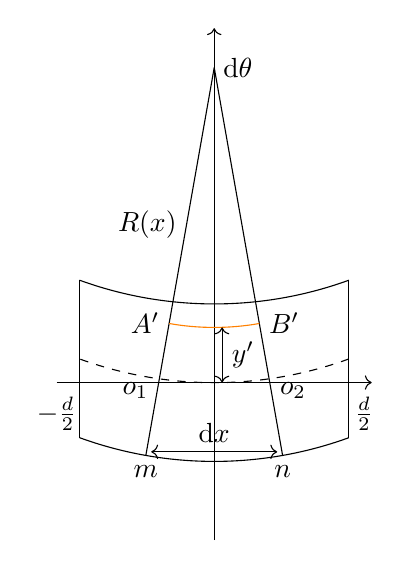
\begin{tikzpicture}
            \draw (1.71,0.3) arc (290:250:5);
            \draw (1.71,2.3) arc (290:250:5);
            %\draw (0,5)--(1,5);
            \draw (1.71,0.3)--(1.71,2.3);
            \draw (-1.71,0.3)--(-1.71,2.3);
            \draw (0.8682,0.0760)node[below]{$ n $} -- (0,5);
            \draw (-0.8682,0.0760)node[below]{$ m $} -- (0,5);
            \draw[->] (0,-1)--(0,5.5);
            \draw[->] (-2,1)--(2,1);
            \draw[dashed] (1.71,1.3) arc (290:250:5);
            \draw[<->] (-0.8,0.12)--node[above]{$ \mathrm{d} x $} (0.8,0.12);
            \node at(1.9,0.6) {$ \frac d2 $};
            \node at(-2,0.6) {$ -\frac d2 $};
            \node at(-1,0.9) {$ o_1 $};
            \node at(1,0.9) {$ o_2 $};
            \node at(-0.85,3) {$ R(x) $};
            \node at(0.3,5) {$ \mathrm{d}\theta $};
            \draw[orange] (0.573,1.7501) arc (280:260:3.3);
            \node[left] at(-0.573,1.7501) {$ A' $};
            \node[right] at(0.573,1.7501) {$ B' $};
            \draw[<->] (0.1,1)--node[right]{$ y' $} (0.1,1.7);
        \end{tikzpicture}
    }
    \caption{弯曲法测杨氏模量原理示意图}
\end{figure}



$ o_1o_2 $所在平面为中性面,既不拉伸也不压缩,$ AB $为距中性面距离$ y $处的平面。变形前有$ o_1o_2=AB=\mathrm{d} x $,变形后则为$ o_1o_2=\mathrm{d} x=R(x)\mathrm{d}\theta,\;A'B'=(R(x)-y)\mathrm{d}\theta $.

那么$ AB $面的应变为
\begin{equation}
\varepsilon=\frac{A'B'-AB}{AB}=\frac{(R(x)-y)\mathrm{d}\theta-\mathrm{d} x}{\mathrm{d} x}=\frac{(R(x)-y)\dfrac{\mathrm{d} x}{R(x)}-\mathrm{d} x}{\mathrm{d} x}=-\frac{y}{R(x)}
\end{equation}
根据胡克定律$ \frac{\mathrm{d} F}{\mathrm{d} S}=Y\varepsilon=-Y\frac{y}{R(x)} $且$ \mathrm{d} S=b\mathrm{d} y $,因此有
\begin{equation}
\mathrm{d} F(x)=-\frac{Y\mathrm{d} y}{R(x)}\mathrm{d} y
\end{equation}
对中性面的转矩为
\begin{equation}\label{2-1}
    \mathrm{d}\mu(x)=|\mathrm{d} F(x)|y=\frac{Yb}{R(x)}y^2\mathrm{d} y
\end{equation}
积分可得
\begin{equation}
\mu(x)=\int_{-a/2}^{a/2}\frac{Yb}{R(x)}y^2\mathrm{d} y=\frac{Yba^3}{12R(x)}
\end{equation}
对梁上各点有$ \frac{1}{R(x)}=\frac{y''(x)}{[1+y'(x)]^{3/2}} $,由于梁的弯曲很小,$ y'(x)=0 $,所以
\begin{equation}\label{2-2}
    R(x)=\frac{1}{y''(x)}
\end{equation}
在平衡时,梁在$ x $处的转矩应与梁右端支撑力$ \frac{Mg}{2} $对$ x $处的力矩平衡,因此有
\begin{equation}\label{2-3}
    \mu(x)=\frac{Mg}{2}\left(\frac d2-x\right)
\end{equation}
由(\ref{2-1}),(\ref{2-2}),(\ref{2-3})可得
\begin{equation}
y''(x)=\frac{6Mg}{Yba^3}\left(\frac d2-x\right)
\end{equation}
代入边界条件$ y(0)=0,\;y'(0)=0 $可求得
\begin{equation}
y(x)=\frac{3Mg}{Yba^3}\left(\frac d2x^2-\frac13x^3\right)
\end{equation}
在中点$ x=\frac d2 $处,有
\begin{equation}
\Delta z=y\left(\frac d2\right)=\frac{Mgd^3}{4Yba^3}
\end{equation}
所以杨氏模量为
\begin{equation}\label{2}
    Y=\frac{d^3Mg}{4a^3b\Delta Z}
\end{equation}
其中$ d $为两刀口间的距离,$ M $为所加拉力对应的质量,$ a $为梁的厚度,$ b $为梁的宽度,$ \Delta Z $为梁中心由于外力作用而下降的距离,$ g $为重力加速度。

\subsection{实验注意事项}
\begin{enumerate}
\item 用千分尺待测样品厚度必须不同位置多点测量取平均值,并且测量黄铜时,用力需适度。

\item 用读数显微镜测量铜刀口基线位置时,刀口不能晃动。

\item 调整霍尔传感器水平,并对各种元件作位置检查和数字归零处理,

\item 实验结束后,关闭电源,整理实验桌面,实验器材放置于实验初始位置。
\end{enumerate}

\subsection{实验步骤}

\begin{enumerate}
\item 调平——首先用水平泡观察平台是否处于水平位置, 若偏离时调节下方水平调节机脚. 

\item 实验装置的调整——大致安装好实验仪器的相对位置,通过磁体调节结构上下移动磁铁使集成霍尔位置传感器探测元件处于磁铁中间的位置(此处磁场可视为均匀).
调节好后固定,最后在拉力绳不受力的情况下将电子称传感器加力系统进行调零.


\item 调节读数显微镜——轻微转动或调整使眼睛观察到清晰的十字线及分划板刻度线和数字. 然后移动读数显微镜前后距离, 直到
清晰看到铜刀口上的黑色基线. 使用适当的力锁紧加力旋钮旁边的锁紧螺钉, 转动读数显微镜读数鼓轮使
铜刀口上的基线与读数显微镜内十字刻度线吻合.

\item 读取数据——通过加力调节旋钮逐次增加拉力 (每次增加10g) , 相应从读数显微镜上读出梁的弯曲位移$\Delta Z_i$及霍尔数
字电压表相应的读数值$U_i$(单位 mV) . 以便计算杨氏模量和对霍尔位置传感器进行定标.

\item 测量几何尺寸——实验完毕松开加力旋钮旁边的锁紧螺钉, 松开加力旋钮, 取下样品.接着多次测量并记录试样在两刀口间的长度 d、不同位置黄铜宽度 b 以及黄铜厚度 a.

\item 整理实验桌面——关闭电源, 整理实验桌面, 实验器材放置于实验初始位置.
\end{enumerate}

\subsection{数据处理}

\subsubsection*{4.5.1 \ \ 黄铜样品}

黄铜样品的几何尺寸测量数据见表 \ref{黄铜样品几何尺寸测量数据},实验时的霍尔测量数据见表 \ref{黄铜样品霍尔测量数据},其中显微镜初始读数为 $Z_0 = 1.011 \ \mathrm{mm}$。下面进行一些数据处理,首先计算黄铜样品几何尺寸的不确定度:
\begin{gather}
u_A(d) = \sqrt{\frac{\sum_{i=1}^{6}\left(d_i - \overline{d}\right)^2}{6\times (6 - 1)}} ,\quad u_{B2}(d) = \frac{e}{\sqrt{3}} \Longrightarrow u(d) = \sqrt{u_A^2(d) + u_{B2}^2(d)} = 0.1750 \ \mathrm{mm} \\
u_A(b) = \sqrt{\frac{\sum_{i=1}^{6}\left(b_i - \overline{b}\right)^2}{6\times (6 - 1)}} ,\quad u_{B2}(b) = \frac{e}{\sqrt{3}} \Longrightarrow u(b) = \sqrt{u_A^2(b) + u_{B2}^2(b)} = 0.0176 \ \mathrm{mm} \\ 
u_A(a) = \sqrt{\frac{\sum_{i=1}^{6}\left(a_i - \overline{a}\right)^2}{6\times (6 - 1)}} ,\quad u_{B2}(a) = \frac{e}{\sqrt{3}} \Longrightarrow u(a) = \sqrt{u_A^2(a) + u_{B2}^2(a)} = 0.0038 \ \mathrm{mm}
\end{gather}
因此黄铜样品的几何尺寸为:
\begin{gather}
    d = (229.6 \pm 0.2) \ \mathrm{mm},\quad 
    b = (23.47 \pm 0.02) \ \mathrm{mm},\quad  
    a = (0.979 \pm 0.004) \ \mathrm{mm}
\end{gather}

\begin{table}[H]\centering
    %\renewcommand{\arraystretch}{1.5} % 调整行间距为 1.5 倍
    %\setlength{\tabcolsep}{1.5mm} % 调整列间距
    \caption{黄铜样品几何尺寸测量数据}
    \label{黄铜样品几何尺寸测量数据}
\resizebox{\columnwidth}{!}{
    \begin{tabular}{cccccccccc}\toprule
        测量次数 & 1 & 2 & 3 & 4 & 5 & 6 & 均值 & 仪器 & 允差 $e$ \\
        \midrule
        长度 $d$ (mm) & 229.2 & 230.1 & 230.0 & 229.4 & 229.3 & 229.3 &  229.5500 & 毫米直尺 (300 mm) & $\pm$ 0.12 mm \\
        宽度 $b$ (mm) & 23.50 & 23.46 & 23.44 & 23.44 & 23.48 & 23.52 &  23.4733 & 游标卡尺 (50 分度) & $\pm$ 0.02 mm \\
        厚度 $a$ (mm) & 0.980 & 0.983 & 0.979 & 0.965 & 0.980 & 0.986 &  0.9788 & 螺旋测微仪 & $\pm$ 0.004 mm \\ 
        \bottomrule
    \end{tabular}
}
\end{table}
\begin{table}[H]\centering
    %\renewcommand{\arraystretch}{1.5} % 调整行间距为 1.5 倍
    %\setlength{\tabcolsep}{1.5mm} % 调整列间距
    \caption{黄铜样品霍尔测量数据}
    \label{黄铜样品霍尔测量数据}
\begin{tabular}{cccccccccc}\toprule
    序号 $i$ & 1 & 2 & 3 & 4 & 5 & 6 & 7 & 8 & 均值 \\
    \midrule
    $M_i$ (g)& 12.4 & 22.0 & 29.6 & 39.8 & 50.0 & 59.5 & 70.3 & 80.0 &  45.4500 \\
    $Z_i$  (mm) & 1.125 & 1.229 & 1.316 & 1.433 & 1.540 & 1.659 & 1.782 & 1.897 &  1.4976 \\
    $U_i$  (mV) & 34 & 58 & 78 & 104 & 128 & 149 & 175 & 201 &  115.8750 \\ 
    \bottomrule
\end{tabular}
\end{table}


为了能顺利用逐差法计算黄铜样品的杨氏模量,我们还需要确定 $\Delta Z$、$\Delta M$的均值和不确定度。它们都属于多次测量,$n = 4$,显微镜读数允差 $e = \pm 0.002 \ \mathrm{mm}$,拉力读数允差 $e = \pm 0.2 \ \mathrm{g}$,于是:
\begin{gather}
\Delta Z_1 = 0.4150 \ \mathrm{mm},\quad \Delta Z_2 = 0.4300\ \mathrm{mm},\quad \Delta Z_3 = 0.4660 \ \mathrm{mm},\quad \Delta Z_4 = 0.4640 \ \mathrm{mm} \\ 
\Longrightarrow
\overline{\Delta Z} = \frac{1}{4}\sum_{i=1}^{4}\Delta Z_i = 0.4438 \ \mathrm{mm} \\ 
u_A(\Delta Z) = \sqrt{\frac{\sum_{i=1}^{4}\left(\Delta Z_i - \overline{\Delta Z}\right)^2}{4\times (4 - 1)}} ,\quad u_{B2}(\Delta Z) =  \frac{e}{\sqrt{3}} \\ 
\Longrightarrow u(\Delta Z) = \sqrt{u_A^2(\Delta Z) + u_{B2}^2(\Delta Z)} = 0.0127 \ \mathrm{mm} \\ 
\Delta M_i = 37.6 \ \mathrm{g},\ \  37.5 \ \mathrm{g},\ \  40.7 \ \mathrm{g},\ \  40.2\ \mathrm{g} 
\Longrightarrow
\overline{\Delta M} = \frac{1}{4}\sum_{i=1}^{4}\Delta M_i = 39.000 \ \mathrm{g} \\
u_A(\Delta M) = \sqrt{\frac{\sum_{i=1}^{4}\left(\Delta M_i - \overline{\Delta M}\right)^2}{4\times (4 - 1)}} ,\quad u_{B2}(\Delta M) =  \frac{e}{\sqrt{3}} \\
\Longrightarrow u(\Delta M) = \sqrt{u_A^2(\Delta M) + u_{B2}^2(\Delta M)} = 0.8515 \ \mathrm{g}
\end{gather}
不确定度取一位有效数字,得到 $\Delta Z$ 和 $\Delta M$ 的测量结果为:
\begin{equation}
    \Delta Z = (0.44 \pm 0.02) \ \mathrm{mm},\quad 
    \Delta M = (39.0 \pm 0.9) \ \mathrm{g}
\end{equation}


\subsubsection*{4.5.2 \ \ 铸铁样品}


铸铁样品的几何尺寸测量数据见表 \ref{铸铁样品几何尺寸测量数据},实验时的霍尔测量数据见表 \ref{铸铁样品霍尔测量数据},其中显微镜初始读数为 $Z_0 = 0.046 \ \mathrm{mm}$。下面进行一些数据处理,首先计算铸铁样品几何尺寸的不确定度:
\begin{gather}
u_A(d) = \sqrt{\frac{\sum_{i=1}^{6}\left(d_i - \overline{d}\right)^2}{6\times (6 - 1)}} ,\quad u_{B2}(d) = \frac{e}{\sqrt{3}} \Longrightarrow u(d) = \sqrt{u_A^2(d) + u_{B2}^2(d)} = 0.1570 \ \mathrm{mm} \\
u_A(b) = \sqrt{\frac{\sum_{i=1}^{6}\left(b_i - \overline{b}\right)^2}{6\times (6 - 1)}} ,\quad u_{B2}(b) = \frac{e}{\sqrt{3}} \Longrightarrow u(b) = \sqrt{u_A^2(b) + u_{B2}^2(b)} = 0.0624 \ \mathrm{mm} \\ 
u_A(a) = \sqrt{\frac{\sum_{i=1}^{6}\left(a_i - \overline{a}\right)^2}{6\times (6 - 1)}} ,\quad u_{B2}(a) = \frac{e}{\sqrt{3}} \Longrightarrow u(a) = \sqrt{u_A^2(a) + u_{B2}^2(a)} = 0.0035 \ \mathrm{mm}
\end{gather}
因此铸铁样品的几何尺寸为:
\begin{gather}
    d = (229.7 \pm 0.2) \ \mathrm{mm},\quad 
    b = (23.34 \pm 0.07) \ \mathrm{mm},\quad  
    a = (0.973 \pm 0.004) \ \mathrm{mm}
\end{gather}

\begin{table}[H]\centering
    %\renewcommand{\arraystretch}{1.5} % 调整行间距为 1.5 倍
    %\setlength{\tabcolsep}{1.5mm} % 调整列间距
    \caption{铸铁样品几何尺寸测量数据}
    \label{铸铁样品几何尺寸测量数据}
\resizebox{\columnwidth}{!}{
    \begin{tabular}{cccccccccc}\toprule
        测量次数 & 1 & 2 & 3 & 4 & 5 & 6 & 均值 & 仪器 & 允差 $e$ \\
        \midrule
        长度 $d$ (mm) & 229.4 & 230.0 & 229.5 & 229.5 & 229.8 & 230.1 &  229.7167 & 毫米直尺 (300 mm) & $\pm$ 0.12 mm \\
        宽度 $b$ (mm) & 23.32 & 23.34 & 23.36 & 23.34 & 23.341 & 23.32 &  23.3368 & 游标卡尺 (50 分度) & $\pm$ 0.02 mm \\
        厚度 $a$ (mm) & 0.973 & 0.976 & 0.969 & 0.974 & 0.973 & 0.975 &  0.9733   & 螺旋测微仪 & $\pm$ 0.004 mm \\ 
        \bottomrule
    \end{tabular}
}
\end{table}
\begin{table}[H]\centering
    %\renewcommand{\arraystretch}{1.5} % 调整行间距为 1.5 倍
    %\setlength{\tabcolsep}{1.5mm} % 调整列间距
    \caption{铸铁样品霍尔测量数据}
    \label{铸铁样品霍尔测量数据}
\begin{tabular}{cccccccccc}\toprule
    序号 $i$ & 1 & 2 & 3 & 4 & 5 & 6 & 7 & 8 & 均值 \\
    \midrule
    $M_i$ (g)   & 20.2 & 39.6 & 60.0 & 81.4 & 100.6 & 120.5 & 140.0 & 160.0 &  90.2875 \\
    $Z_i$  (mm) & 0.189 & 0.320 & 0.461 & 0.603 & 0.717 & 0.868 & 1.019 & 1.162 &  0.6674 \\
    $U_i$  (mV) & 31 & 61 & 91 & 122 & 150 & 178 & 205 & 233 &  133.8750 \\
    \bottomrule
\end{tabular}
\end{table}

同样地,为了能顺利用逐差法计算铸铁样品的杨氏模量,我们还需要确定 $\Delta Z$、$\Delta M$ 的均值和不确定度。它们都属于多次测量,$n = 4$,显微镜读数允差 $e = \pm 0.002 \ \mathrm{mm}$,拉力读数允差 $e = \pm 0.2 \ \mathrm{g}$,于是:
\begin{gather}
\Delta Z_1 = 0.5280 \ \mathrm{mm},\quad \Delta Z_2 = 0.5480\ \mathrm{mm},\quad \Delta Z_3 = 0.5580 \ \mathrm{mm},\quad \Delta Z_4 = 0.5590 \ \mathrm{mm} \\ 
\Longrightarrow
\overline{\Delta Z} = \frac{1}{4}\sum_{i=1}^{4}\Delta Z_i = 0.5482 \ \mathrm{mm} \\ 
u_A(\Delta Z) = \sqrt{\frac{\sum_{i=1}^{4}\left(\Delta Z_i - \overline{\Delta Z}\right)^2}{4\times (4 - 1)}} ,\quad u_{B2}(\Delta Z) =  \frac{e}{\sqrt{3}} \\ 
\Longrightarrow u(\Delta Z) = \sqrt{u_A^2(\Delta Z) + u_{B2}^2(\Delta Z)} = 0.0073 \ \mathrm{mm} 
\\ 
\Delta M_i = 80.4 \ \mathrm{g},\ \  80.9 \ \mathrm{g},\ \  80.0 \ \mathrm{g},\ \  78.6\ \mathrm{g} 
\Longrightarrow
\overline{\Delta M} = \frac{1}{4}\sum_{i=1}^{4}\Delta M_i = 79.975 \ \mathrm{g} \\ 
u_A(\Delta M) = \sqrt{\frac{\sum_{i=1}^{4}\left(\Delta M_i - \overline{\Delta M}\right)^2}{4\times (4 - 1)}} ,\quad u_{B2}(\Delta M) =  \frac{e}{\sqrt{3}}
\end{gather}
\begin{gather}
    \Longrightarrow u(\Delta M) = \sqrt{u_A^2(\Delta M) + u_{B2}^2(\Delta M)} = 0.5072 \ \mathrm{g}
\end{gather}

不确定度取一位有效数字,得到 $\Delta Z$ 和 $\Delta M$ 的结果为:
\begin{equation}
    \Delta Z = (0.548 \pm 0.008) \ \mathrm{mm},\quad
    \Delta M = (80.0 \pm 0.6) \ \mathrm{g}
\end{equation}

\subsection{实验结果}

\subsubsection*{4.6.1 \ \ 逐差法}

对于黄铜样品,已有的数据如下:
\begin{gather}
    d = (229.6 \pm 0.2) \ \mathrm{mm},\quad
    b = (23.47 \pm 0.02) \ \mathrm{mm},\quad
    a = (0.979 \pm 0.004) \ \mathrm{mm}\\ 
    \Delta Z = (0.44 \pm 0.02) \ \mathrm{mm},\quad 
    \Delta M = (39.0 \pm 0.9) \ \mathrm{g},\quad
    g = 9.807 \ \mathrm{m/s^2}
\end{gather}
代入公式 (\ref{2}),可得黄铜样式模量的实验值 $Y$,进一步与讲义上的标准数据 $Y_0 = 10.55  \times 10^{10} \ \mathrm{N\cdot m^{-2}} $ 作比较,得到相对误差 $\eta$。结果如下:
\begin{gather}
    \overline{Y} = \frac{d^3 g \Delta M}{4a^3b\Delta Z} = 11.839 \times 10^{10} \ \mathrm{N\cdot m^{-2}} \\ 
    u(Y) = \overline{Y} \cdot \sqrt{
    \left[ 3 \frac{u(d)}{d} \right]^2 + 
    \left[\frac{u(\Delta M)}{\Delta M}\right]^2 + 
    \left[ 3 \frac{u(a)}{a} \right]^2 + 
    \left[ \frac{u(b)}{b} \right] + 
    \left[ \frac{u(\Delta Z)}{\Delta Z} \right]^2
    } =  0.1392 \times 10^{10} \ \mathrm{N\cdot m^{-2}} \\
    \Longrightarrow \text{黄铜:}  \boldsymbol{
        Y = \overline{Y} \pm u(Y) = (11.8 \pm 0.2) \times 10^{10} \ \mathrm{N\cdot m^{-2}}
        ,\quad 
        \eta = 12.2227 \%
    }
\end{gather}

对于铸铁样品,已有的数据如下:
\begin{gather}
    d = (229.7 \pm 0.2) \ \mathrm{mm},\quad
    b = (23.34 \pm 0.07) \ \mathrm{mm},\quad
    a = (0.973 \pm 0.004) \ \mathrm{mm}\\ 
    \Delta Z = (0.548 \pm 0.008) \ \mathrm{mm},\quad 
    \Delta M = (80.0 \pm 0.6) \ \mathrm{g},\quad
    g = 9.807 \ \mathrm{m/s^2}
\end{gather}
代入公式 (\ref{2}),可得铸铁样式模量的实验值 $Y$,进一步与讲义上的标准数据 $Y_0 = 18.15  \times 10^{10} \ \mathrm{N\cdot m^{-2}} $ 作比较,得到相对误差 $\eta$。结果如下:
\begin{gather}
    \overline{Y} = \frac{d^3 g \Delta M}{4a^3b\Delta Z} = 20.147 \times 10^{10} \ \mathrm{N\cdot m^{-2}} \\ 
    u(Y) = \overline{Y} \cdot \sqrt{
    \left[ 3 \frac{u(d)}{d} \right]^2 + 
    \left[\frac{u(\Delta M)}{\Delta M}\right]^2 + 
    \left[ 3 \frac{u(a)}{a} \right]^2 + 
    \left[ \frac{u(b)}{b} \right] + 
    \left[ \frac{u(\Delta Z)}{\Delta Z} \right]^2
    } =  0.3373 \times 10^{10} \ \mathrm{N\cdot m^{-2}} \\
    \Longrightarrow \text{铸铁:} \boldsymbol{
        Y = \overline{Y} \pm u(Y) = (20.1 \pm 0.4) \times 10^{10} \ \mathrm{N\cdot m^{-2}}
        ,\quad 
        \eta = 11.0008 \%
    }
\end{gather}


\subsubsection*{4.6.2 \ \ 最小二乘法}

按老师的要求,本实验需要用最小二乘法和画图法对霍尔位置传感器定标,也即计算霍尔传感器的灵敏度,这等价于 $U = U(Z)$ 图像的斜率 $k$。并没有不确定度的计算要求。

由最小二乘法的公式,可得:
\begin{gather}
\text{黄铜数据:} k = 
\frac{\sum_{i=1}^{8} \left( U_i - \overline{U}\right) \left(Z_i - \overline{Z}\right) }{ \sum_{i=1}^{8}\left(Z_i - \overline{Z}\right)^2 } = 213.7411 \ \mathrm{mV \cdot mm^{-1}} \\ 
\text{铸铁数据:} k = \frac{\sum_{i=1}^{8} \left( U_i - \overline{U}\right) \left(Z_i - \overline{Z}\right) }{ \sum_{i=1}^{8}\left(Z_i - \overline{Z}\right)^2 } = 207.9053  \ \mathrm{mV \cdot mm^{-1}} 
\end{gather}

\subsubsection*{4.6.3 \ \ 作图法}

选取拟合函数为 $y = ax + b$,在这里即 $ U = kZ + U_0$,在 Matlab 软件中,用 Bisquare 算法对原数据进行拟合,得到拟合结果与优度:
\begin{gather}
\text{黄铜数据:} 
\begin{cases}
    k =   213.6172 \ \mathrm{mV \cdot mm^{-1}} 
    \\ 
    R^2 = 0.9988,\quad  \text{SSE} = 28.5691 \ \mathrm{mV^2},\quad \text{RMSE} = 2.1821 \ \mathrm{mV}
\end{cases}
\\
\text{铸铁数据:} 
\begin{cases}
    k = 207.9050 \ \mathrm{mV \cdot mm^{-1}} 
    \\ 
    R^2 = 0.9974,\quad  \text{SSE} = 90.5856 \ \mathrm{mV^2},\quad \text{RMSE} = 3.8856 \ \mathrm{mV}
\end{cases}
\end{gather}
在坐标系中分别作出两种样品数据下,$U = U(Z)$ 随 $Z$ 的变化情况,如下图所示:
\begin{figure}[H]\centering
\begin{subfigure}[b]{0.48\columnwidth}\centering
    \includegraphics[height=182pt]{assets/2 霍尔/黄铜.pdf}
    \caption{黄铜样品数据}
\end{subfigure}\hfill
\begin{subfigure}[b]{0.50\columnwidth}\centering
    \includegraphics[height=182pt]{assets/2 霍尔/铸铁.pdf}
    \caption{铸铁样品数据}
\end{subfigure}
\caption{作图法求霍尔位移传感器灵敏度}
\end{figure}


\section{动态悬挂法}
\subsection{实验仪器与用具}
DHY-2A 型动态杨氏模量测试台、DH0803 振动力学通用信号源,
通用示波器、
测试棒(铜、不锈钢)、悬线、专用连接导线、天平、游标卡尺、螺旋测微计等。

\begin{figure}[H]\centering
    \includegraphics[width=0.75\columnwidth]{assets/0/a36e12208fcd72455f93e4b950ef3249.png}
    \caption{DHY-2A 型动态杨氏模量测试装置}
\end{figure}

\subsection{实验原理}

先令$y$为棒振动的位移,$Y$为棒振动的杨氏模量,$S$为棒的横截面积,$J$为棒的转动惯量,$\rho$为棒密度,$x$为位置坐标,$t$为时间变量
通过分离变数法,即令$y(x,t)=X(x)T(t)$,可解得
\begin{equation}
    y(x,t)=\left(A_1{\rm ch}K_x+A_2{\rm sh}K_x+B_1\cos K_x+B_2\sin K_x \right)\cos (\omega t+\varphi)
\end{equation}
其中$\omega= \sqrt{\frac{K^4YJ}{\rho S}}$称为频率公式,$K$为常数,$A_1,A_2,B_1,B_2,\varphi$为待定常数,可由边界和初始条件确定。

对于长为$L$,两端自由的棒,当悬线悬挂于棒的节点附近时,其边界条件为:
自由端横向作用力$F$为零,弯矩$M$亦为零:
\begin{equation}
   F=-\frac{\partial M}{\partial x} =0\qquad 
   M=EJ\frac{\partial^2y}{\partial x^2}=0
\end{equation}

将边界条件带入通解$y=(x,t)$中可的超越方程$\cos KL\cdot {\rm ch}KL=1$.
其第一个根为$0$,对应于静态值,第二个根 $K_1L\approx 4.7300$,此时的共振频率称为基频 (或固有频率) $\omega_1=2\pi f_1$。
对于直径为$d$,长为$L$,质量为$m$的圆形棒,可知在此频率下共振时,其杨氏模量:
\begin{equation}\label{3}
   Y=1.6067 \cdot \frac{L^3mf_1^2}{d^4} 
\end{equation}

测试棒在作基频振动时存在两个节点,它们的位置距离端面 $0.224L $(距离另一端面为 $0.776 L$ )
处,理论上,悬挂点应取在节点处测试棒难于被激振和拾振,为此可在节点两旁选不同点对称悬挂,用外推法找出节点处的共振频率。

\subsection{实验注意事项}

\begin{enumerate}
\item 本实验中只能测出的共振频率。但由于二者相差很小,故固有频率可用共振频率代替。

\item 安装测试棒时,应先移动支架到既定位置,再悬挂,需保证横向水平,悬线与测试棒轴向垂直。

\item 在示波器显示出现共振现象之后,需十分缓慢地微调频率调节细调旋钮,使波形振幅达到极大值。

\item 因为设备尺寸原因,部分设备在$0.0365L$、$ 0.9635L$处悬线不能竖直,此时该点要丢弃不测。

\item 每次测量时都用这种方法判别其是否为基频:沿测试棒长度的方向轻触棒的不同部位,观察示波器,在波节处波幅不变化,
而在波腹处,波幅会变小,并发现测试棒上有两个波节。

\end{enumerate}

\subsection{实验步骤}
\begin{enumerate}
\item 正确连接装置。

\item 测量共振频率:待测试棒稳定后,调节信号源发出信号的频率和幅度(先粗调再微调,可按照位数从高到低开始调节),寻找测试棒的共振频率:表示为示波器上正弦波幅度最大值(实际过程中变化可能有延迟,需要等待波形稳定后进行判断),并进行数据的记录,重复上述操作。

\item 实验结束后归纳并整理好实验台面。

\end{enumerate}

\subsection{数据处理}

黄铜棒的共振测量数据详见表 \ref{黄铜棒共振频率数据},质量和几何测量参数如下所示:
\begin{equation}
    L = 180.0 \ \mathrm{mm},\quad 
    d = 5.956 \ \mathrm{mm},\quad 
    m = 42.10 \ \mathrm{g}
\end{equation}
\noindent 再讨论上述参量的不确定度,对长度测量,有 $u(x) = \sqrt{2 u_{B1}(x)^2 + u_{B2}(x)^2 } = \sqrt{ 2 \left(\frac{d}{10}\right)^2 + \left(\frac{e}{\sqrt{3}}\right)^2 }$,于是:
\begin{gather}
\text{钢直尺:} d = 1 \ \mathrm{mm},\ e = \pm 0.12 \ \mathrm{mm} \Longrightarrow u(L) = 0.1575 \ \mathrm{mm} = 0.2 \ \mathrm{mm}\\ 
\text{千分尺:} d = 0.01 \ \mathrm{mm},\ e = \pm 0.004 \ \mathrm{mm} \Longrightarrow u(d) =  0.0027 \ \mathrm{mm} = 0.003 \ \mathrm{mm}\\ 
\text{电子称:} d = 0.01 \ \mathrm{g},\ e = \pm 0.01 \ \mathrm{g} \Longrightarrow u(m) = 0.0059 \ \mathrm{g} = 0.006 \ \mathrm{g}
\end{gather}


\begin{table}[H]\centering
    %\renewcommand{\arraystretch}{1.5} % 调整行间距为 1.5 倍
    %\setlength{\tabcolsep}{1.5mm} % 调整列间距
    \caption{黄铜棒共振频率数据}
    \label{黄铜棒共振频率数据}
\begin{tabular}{cccccccccc}\toprule
    序号 & 1 & 2 & 3 & 4 & 5 & 6 & 7 & 8 \\
    \midrule
    悬挂位置 $x$ (mm) & 20 & 25 & 30 & 35 & 45 & 50 & 55 & 60 \\
    $\frac{x}{L}$  & 0.1111 & 0.1389 & 0.1667 & 0.1944 & 0.2500 & 0.2778 & 0.3056 & 0.3333 \\
    共振频率 $f$ (Hz) & 592.696 & 589.847 & 588.386 & 587.325 & 586.789 & 587.759 & 588.798 & 590.082 \\
    \bottomrule
\end{tabular}
\end{table}

\subsection{实验结果 (拟合法)}

由于讲义中并没有给出频率 $f$ 关于悬挂点 $x$ (或 $\frac{x}{L}$) 的变化规律,拟合函数的选取范围是很广的。在综合考虑了拟合效果和物理意义之后,我们选取了四次函数进行拟合,拟合函数如下:
\begin{equation}
    f = f\left(\frac{x}{L}\right) = a\left(\frac{x}{L}\right)^4 + b\left(\frac{x}{L}\right)^^3 + c\left(\frac{x}{L}\right)^2 + d\left(\frac{x}{L}\right) + e 
\end{equation}
其中 $a, b, c, d, e$ 是待定常数。在 Matlab 中,用 Bisquare 算法对原数据进行拟合,得到拟合结果如图 \ref{动态悬挂法求共振频率} 所示,下面是拟合的一些优度参数:
\begin{equation}
R^2 = 0.9941,\quad  \text{SSE} = 0.1487 \ \mathrm{Hz^2},\quad \text{RMSE} = 0.2226 \ \mathrm{Hz}
\end{equation}
\begin{figure}[H]\centering
    \includegraphics[width=0.9\columnwidth]{assets/3 动态/2024-11-13_00-42-44.pdf}
    \caption{动态悬挂法求共振频率 $f_1$}\label{动态悬挂法求共振频率}
\end{figure}
对所得拟合函数求导,可得最小值位于 $x / L = 0.226883$ 处,此时基频共振频率 $f_1$ 为:
\begin{equation}
    \frac{x}{L} = 0.22688279,\quad f_1 = 586.8180 \ \mathrm{Hz}
\end{equation}
受拟合特性本身影响,无法确定频率 $f_1$ 的不确定度,在后续计算中不考虑此项。

再次汇总数据如下:
\begin{equation}
    L = (180.0 \pm 0.2) \ \mathrm{mm},\quad d = (5.956 \pm 0.003) \ \mathrm{mm},\quad m = (42.100 \pm 0.006) \ \mathrm{g}
\end{equation}
代入公式 (\ref{3}),可得黄铜棒的杨氏模量 $Y$ 及其不确定度: 
\begin{gather}
    \overline{Y} = 1.6067 \cdot \frac{L^3 m f_1^2}{d^4} = 10.795 \times 10^{10} \ \mathrm{N\cdot m^{-2}} \\ 
    u(Y) = \overline{Y}\cdot \sqrt{
    \left[ 3 \frac{u(L)}{L} \right]^2 + 
    \left[ \frac{u(m)}{m} \right]^2 + 
    \left[ 4 \frac{u(d)}{d} \right]^2} = 0.034504 \times 10^{10} \ \mathrm{N\cdot m^{-2}} \\
\Longrightarrow \boldsymbol{
    Y = \overline{Y} \pm u(Y) = (10.80 \pm 0.04) \times 10^{10} \ \mathrm{N\cdot m^{-2}}
}
\end{gather}
由讲义可知,黄铜测试棒的杨氏模量在 $8.0 \times 10^{10} \ \mathrm{N\cdot m^{-2}} $ 至 $ 11.0 \times 10^{10} \ \mathrm{N\cdot m^{-2}} $ 之间,这与我们所测得的结果相符。

\section{*光杠杆法}\vspace*{-6mm}
\begin{graybox}
\textbf{注:}按老师要求,此小节实验不在实验内容安排之中。
\end{graybox}

\subsection{实验仪器与用具}
光杠杆测量系统(光杠杆反射镜、倾角调节架、标尺、
望远镜及调节反射镜等)、游标卡尺、螺旋测微器等。

\subsection{实验原理}

实际上就是采取了一种“放大”的思路,如下图所示:
\begin{figure}[H]\centering
    \includegraphics[width=0.6\columnwidth]{assets/0/image (19) copy.png}
    \caption{光杠杆法测量原理}
\end{figure}
当钢丝的长度发生变化时,光杠杆的镜面必然不再竖直,有一角度变化。经过光路放大之后,便得到可以显著测量到的量:
\begin{equation}
    \Delta L=b\tan \theta\quad 2\theta \approx \frac{C/2}{H}
    \quad E=\frac{16FLH}{\pi D^2bC}
\end{equation}
这就得到了我们在本实验中需要依照的公式,其中用到了小角近似。

\subsection{实验注意事项}
\begin{enumerate}
\item 本实验由此需要细致调节:先目测调整之后,在通过调节望远镜的目镜旋轮,使“十”字清晰成像,随后细调光路至水平。
\item 注意测量中的误差记录与分析,并多次测量求平均以尽可能达到最佳的实验精度。

\end{enumerate}

\section{思考题}

\subsection*{7.1 \quad  拉伸法}
\subsubsection*{7.1.1 \ \ 杨氏模量测量数据 $N$ 若不用逐差法而用作图法,如何处理?}
以砝码总质量 $M$ (g) 为横坐标,变化的长度 $\Delta L$ (mm) 为纵坐标,在坐标轴上作出所测得的数据。丢弃极端数据后,用直线尽可能逼近各离散点,使得尽量多的点落在直线上,不在直线上的点也均匀分布在直线两侧。然后算出直线的斜率 $k$,即可换算得到杨氏模量 $Y=\frac{4gL}{k\pi d^2}$。

\subsubsection*{7.1.2 \ \ 两根材料相同但粗细不同的金属丝,它们的杨氏模量相同吗?为什么?}
它们杨氏模量是相同的。杨氏模量是材料的固有性质,它体现材料抗应变的能力,其大小只由材料的性质决定,与材料的几何参数无关。

\subsubsection*{7.1.3 \ \ 本实验使用了哪些测量长度的量具?选择它们的依据是什么?它们的仪器误差各是多少?}
下表列出了本实验所使用到的长度量具,以及它们的测量误差:
\begin{table}[H]\centering
    %\renewcommand{\arraystretch}{1.5} % 调整行间距为 1.5 倍
    %\setlength{\tabcolsep}{1.5mm} % 调整列间距
    \caption{本次实验用到的长度量具及其误差}
    \label{本次实验用到的长度量具及其误差}
\begin{tabular}{cccccccccc}\toprule
    名称 & 量程 & 分度值 & 允差  \\
    \midrule
    钢直尺 & 300 mm & 1 mm & $\pm$ 0.12 mm \\
    钢卷尺 & 3 m & 1 mm & $\pm$ 2.0 mm \\
    游标卡尺 & 125 mm & 0.02 mm & $\pm$ 0.02 mm \\
    螺旋测微仪 & 25 mm & 0.01 mm & $\pm$ 0.004 mm \\
    拉伸法电子刻度线 & 4 mm & 0.05 mm & $\pm$ 0.005 mm \\
    弯曲法电子刻度线 & 6 mm & 0.01 mm  & $\pm$ 0.002 mm  \\
    \bottomrule
\end{tabular}
\end{table}
同时考虑了量程、精度(包括不确定度)和方便程度,所以选择上述仪器。

\subsubsection*{7.1.4 \ \ 在 CCD 法测定金属丝杨氏模量实验中,为什么起始时要加一定数量的底码?}
未加砝码的情形下,金属丝不一定伸直,可能会有轻微弯折。若忽略了这部分弯折带来的影响,加力后弯折部分被拉直,产生不是由钼丝本身伸缩导致的伸长,增大了实验误差。
因此,在开始实验之前,需要加适量的砝码,将钼丝尽可能拉直,以保证测量的准确性。

\subsubsection*{7.1.5 \ \ 加砝码后标示横线在屏幕上可能上下颤动不停,不能够完全稳定时,如何判定正确读数?}
待其稳定后读数即可。如等待较长时间仍不稳定,可以用手轻轻控制,使其稳定下来,再行读数。


\subsubsection*{7.1.6 \ \ 金属丝存在折弯使测量结果如何变化?}
会杨氏模量的测定结果偏小。金属弯折会导致测得的劲度系数发生变化,导致测得的整体劲度系数变小,从而使 $\Delta l$ 偏大。由公式 $Y = \frac{4\Delta MgL}{\pi d^{2}\Delta\bar{l}}$ 可知,最后测量结果将偏小。

\subsubsection*{7.1.7 \ \ 用螺旋测微器或游标卡尺测量时,若初状态都不在零位,需要减去初值,对测量值的误差有何影响?}
这样相当于对数值测量两次后相减,会增大数据的不确定度,具体表现为:
\begin{gather}
\text{读数一次:} u(x) = \sqrt{u_{B1}(x)^2 + u_{B2}(x)^2 },\quad 
\text{读数两次:} u(x) = \sqrt{2u_{B1}(x)^2 + u_{B2}(x)^2 }
\end{gather}

\subsection*{7.2 \quad  霍尔法 (弯曲法)}
\subsubsection*{7.2.1 \ \ 弯曲法测杨氏模量实验,主要测量误差有哪些?请估算各因素的不确定度。}
\noindent 可能的误差来源有:
\begin{enumerate}
\item 测量样品几何尺寸带来的误差:包括长度 $L$、宽度 $b$ 和厚度 $a$;
\item 仪器拉力(质量)示数不稳定:可能未等待示数稳定就行读数,此时的读数便不是准确值;
\item 显微镜读数时的误差:显微镜内十字比样品上的刻线要细,读数时可能会有一定的视觉误差;
\end{enumerate}
在数据处理一节中,我们已经对这些因素的不确定度进行了计算,具体数值如下:
\begin{gather}
\text{黄铜:}
\begin{cases}
    u(L) = 0.2 \ \mathrm{mm},\quad u(b) = 0.02 \ \mathrm{mm},\quad u(a) = 0.004 \ \mathrm{mm} \\
    u(\Delta Z) = 0.02 \ \mathrm{mm},\quad u(\Delta M) = 0.9 \ \mathrm{g} \\ 
\end{cases}
\\
\text{铸铁:}
\begin{cases}
    u(L) = 0.2 \ \mathrm{mm},\quad u(b) = 0.07 \ \mathrm{mm},\quad u(a) = 0.004 \ \mathrm{mm} \\
    u(\Delta Z) = 0.008 \ \mathrm{mm},\quad u(\Delta M) = 0.6 \ \mathrm{g} \\ 
\end{cases} 
\end{gather}

\subsubsection*{7.2.1 \ \ 用霍尔位置传感器法测位移有什么优点?}
霍尔位置传感器法测位移的优点包括:
\begin{enumerate}
\item 高灵敏度:霍尔传感器对磁场变化非常敏感,可以检测到微小的位移变化。
\item 非接触测量:霍尔传感器可以实现非接触测量,避免了机械磨损和摩擦带来的误差。
\item 高精度:在适当的磁场和电流条件下,霍尔传感器可以提供高精度的位移测量。
\end{enumerate}
特别地,与拉伸法中的测量方法相比,霍尔法只需搭建好仪器后调节旋钮,即可改变力的大小,不需手动添加砝码,操作更简便。并且数据以电子方式直接显示在屏幕上,便于记录和处理,也减小了人为读数带来的误差。


\subsection*{7.3 \quad  动态悬挂法}
\subsubsection*{7.3.1 \ \ 外延测量法有什么特点?使用时应注意什么问题?}
外推法是基于已有数据,选择合适、合理而科学的拟合函数进行拟合,以对不便测量或根本无法测量的数据进行拟合或预测的方法。特别是在理论与实际符合得很好的数据中,外推法(拟合法)具有非常高的准确性和说服力。

使用外推法需要注意以下几点:
\begin{enumerate}
\item 丢弃异常值:在拟合之前,应先对数据进行处理,丢弃异常值,保留合理的数据。
\item 若数据分布不均匀,数据间误差较大,外推法的精度将大大降低。因为外推法结果的可靠性直接受已测数据精度影响。
\item 选择合适的拟合函数:拟合函数的选择应基于数据背后的物理原理,符合实际情况,能够较好地拟合已有数据。
\end{enumerate}

\subsubsection*{7.3.1 \ \ 物体的固有频率和共振频率有什么不同?它们之间有何关系?}
固有频率 $f_0$ 是由材料本身的性质决定的,而共振频率 $f_1$ 与具体的实验条件有关,不同的实验条件下,共振频率也常常不相同。两者的关系为:
\begin{equation}
f_0 = f_1 \cdot \sqrt{ 1 + \frac{1}{4Q^2} }
\end{equation}
讲义中提到,对于本次的悬挂法测量,$Q$ 的最小值约为 $50$,这时共振频率 $f_1$ 只比固有频率 $f_0$ 低 $0.005 \%$ 左右。两者相差极小,因此固有频率可用共振频率代替。

\section{实验总结与心得体会}
此次“杨氏模量”实验共分为三个部分(光杠杆部分不作要求),总的来讲都是依据杨氏模量的特性来设计实验,测出杨氏模量的实验值,并与理论值(标准值)作对比。实验的一大重点是“微小量的测量”,我们在不同的部分,使用了不同的小位移(长度)测量工具,令我印象深刻;另一重点是数据不确定度与误差分析,是本次实验报告的重点,在处理的过程中,我也学到很多。

实验总体上是成功的,每个小节的实验都大致符合理论,实验数据和图像也具有较强的说服力。但实际值与理论(标准)值仍有一定的偏差,例如拉伸法的杨氏模量误差达到约 36 \%,这可能是由于实验中的一些细节问题,如实验环境、仪器精度、人为误差等。如何减小这些误差,提高实验的准确性,可能需要进一步的探讨。当然,也不排除样品钼丝的杨氏模量不符合讲义标准值的可能。

特别地,本次实验我利用了 Matlab 软件对实验数据作进一步的处理和分析,包括换算、拟合、可视化等,相比于常规数据处理和画图方法,这大大提高了数据分析处理的速度的准确度,也提高了作图的美观性。在今后的实验和研究工作中,我还会继续深入学习和应用类似地计算软件,增强自己的科学计算能力。科研不是考试,我们应该充分利用好自己能接触到的资源,合理使用工具,更高效地发展自身。

另外,这次实验让我感受到,实验“结束”并不意味着实验就已经完成,事实上这仅是数据测量的结束。在课后,我们还需要重新整理实验原理和过程,换算、分析、拟合实验数据,作出合适的数据图,解释可能存在的误差等。在根据已有数据求所需结果时,如何才能最大程度地利用已有数据,同时又尽可能地降低二次误差。上面这些内容都需要体现在最终的实验报告中,一点点累加起来,着实花费了我很多精力。

但最后,回过头来,我认为一切都是值得的。当处理完毕的结果有力地验证了理论值时,当实验数据图像与理论较好地契合时,心中便迸发出无尽的喜悦,也深深感受到物理“理论与实验结合”的魅力。\footnote{原始数据记录表和部分 Matlab 源码附在附录中。}














\newpage
\section*{附录 A\hspace*{20pt} 原始数据记录表}
\addcontentsline{toc}{section}{附录 A\hspace*{6pt} 原始数据记录表} 
\thispagestyle{fancy} 

\begin{figure}[H]\centering
    \includepdf[pages=1, width=480pt]{pdf/原始数据-2-05组-丁毅-杨氏模量-2024.11.12-董政.pdf}
\end{figure}
\includepdf[pages={2}]{pdf/原始数据-2-05组-丁毅-杨氏模量-2024.11.12-董政.pdf}
\includepdf[pages={3}]{pdf/原始数据-2-05组-丁毅-杨氏模量-2024.11.12-董政.pdf}
\includepdf[pages={4}]{pdf/原始数据-2-05组-丁毅-杨氏模量-2024.11.12-董政.pdf}
% \includepdf[pages={2-4}] 出现了大小不匹配的问题,所以只能分开插入

\section*{附录 B\hspace*{20pt} Matlab 源码}
\addcontentsline{toc}{section}{附录 B\hspace*{6pt} Matlab 源码} 
\thispagestyle{fancy} 
\lstinputlisting{d:/a_RemoteRepo/GH.MatlabCodes/本科课程代码/基础物理实验/Ex_1/Ex_1_mflie.m}



\end{document}

% VScode 常用快捷键:

% F2:                       变量重命名
% Ctrl + Enter:             行中换行
% Alt + up/down:            上下移行
% 鼠标中键 + 移动:           快速多光标
% Shift + Alt + up/down:    上下复制
% Ctrl + left/right:        左右跳单词
% Ctrl + Backspace/Delete:  左右删单词    
% Shift + Delete:           删除此行
% Ctrl + J:                 打开 VScode 下栏(输出栏)
% Ctrl + B:                 打开 VScode 左栏(目录栏)
% Ctrl + `:                 打开 VScode 终端栏
% Ctrl + 0:                 定位文件
% Ctrl + Tab:               切换已打开的文件(切标签)
% Ctrl + Shift + P:         打开全局命令(设置)

% Latex 常用快捷键:

% Ctrl + Alt + J:           由代码定位到PDF


